%The programmer is in the unique position that his [sic] is the only discipline and profession in which such a gigantic ration, which totally baffles out imagination has to be bridges by a single technology.  He [sic] has to be able to think in terms of conceptual hierarchies that are much deeper than a single mind ever needed to face before

\chapter{Data}\label{ch:data}

\chapquotew{From a bit to a few hundred megabytes, from a microsecond to half an hour of computing confronts us with the completely baffling ratio of 10\textsuperscript{9}!  .... By evoking the need for deep conceptual hierarchies, the automatic computer confronts us with a radically new intellectual challenge that has no precedent in our history.}{Edsger Dijkstra\cut{, \emph{The Cruelty of Really Teaching Computer Science} (EWD 1036), 1988.}}{11.5cm}\index{people}{Dijkstra, Edsger}

%\topics{the digital abstraction, measuring information, simple data representation, lists, programming with lists}

For all the programs so far, we have been limited to simple data such as numbers and Booleans.  We call this \definition{scalar} data since it has no structure.  As we saw in Chapter~\ref{ch:intro}, we can represent all discrete data using just (enormously large) whole numbers.  For example, we could represent the text of a book using only one (very large!) number, and manipulate the characters in the book by changing the value of that number.  But, it would be very difficult to design and understand computations that use numbers to represent complex data.  

We need more complex data structures to better model structured data.  We want to represent data in ways that allow us to think about the problem we are trying to solve, rather than the details of how data is represented and manipulated.  

This chapter covers techniques for building data structures and for defining procedures that manipulate structured data, and introduces data abstraction as a tool for managing program complexity. 

\begin{schemeregion}

\section{Types}\label{sec:types}\index{general}{types}\index{general}{Boolean}\index{general}{Number}

All data in a program has an associated type.  Internally, all data is stored just as a sequence of bits, so the type of the data is important to understand what it means.  We have seen several different types of data already: Numbers, Booleans, and Procedures (we use initial capital letters to signify a datatype).  

A \definition{datatype} defines a set (often infinite) of possible values.  The Boolean datatype contains the two Boolean values, \scheme|true| and \scheme|false|.  The Number type includes the infinite set of all whole numbers (it also includes negative numbers and rational numbers).  We think of the set of possible Numbers as infinite, even though on any particular computer there is some limit to the amount of memory available, and hence, some largest number that can be represented.  On any real computer, the number of possible values of any data type is always finite.  But, we can imagine a computer large enough to represent any given number.

The type of a value determines what can be done with it.  For example, a Number can be used as one of the inputs to the primitive procedures \scheme|+|, \scheme|*|, and \scheme|=|.  A Boolean can be used as the first subexpression of an if expression and as the input to the \scheme|not| procedure (|not| can also take a Number as its input, but for all Number value inputs the output is \schemeresult|false|), but cannot be used as the input to \scheme|+|, \scheme|*|, or \scheme|=|.\footnote{The primitive procedure \scheme|equal?| is a more general comparison procedure that can take as inputs any two values, so could be used to compare Boolean values.  For example, \scheme|(equal? false false)| evaluates to \schemeresult|true| and \scheme|(equal? true 3)| is a valid expression that evaluates to \scheme|false|.}  

\index{general}{procedure}
A Procedure can be the first subexpression in an application expression.  There are infinitely many different types of Procedures, since the type of a Procedure depends on its input and output types.  For example, recall \scheme|bigger| procedure from Chapter~\ref{ch:programming}:\index{general}{bigger}
\begin{schemedisplay}
(define (bigger a b) (if (> a b) a b))
\end{schemedisplay}
It takes two Numbers as input and produces a Number as output.  We denote this type as:
\begin{center}
Number $\times$ Number $\rightarrow$ Number 
\end{center}
The inputs to the procedure are shown on the left side of the arrow.  The type of each input is shown in order, separated by the $\times$ symbol.\footnote{The notation using $\times$ to separate input types makes sense if you think about the number of different inputs to a procedure.  For example, consider a procedure that takes two Boolean values as inputs, so its type is Boolean $\times$ Boolean $\rightarrow$ Value.  Each Boolean input can be one of two possible values.  If we combined both inputs into one input, there would be $2 \times 2$ different values needed to represent all possible inputs.}  The output type is given on the right side of the arrow.  

From its definition, it is clear that the \scheme|bigger| procedure takes two inputs from its parameter list.  How do we know the inputs must be Numbers and the output is a Number?

The body of the \scheme|bigger| procedure is an if expression with the predicate expression \scheme|(> a b)|.  This applies the \scheme|>| primitive procedure to the two inputs.  The type of the \scheme|>| procedure is Number $\times$ Number $\rightarrow$ Boolean.  So, for the predicate expression to be valid, its inputs must both be Numbers.  This means the input values to \scheme|bigger| must both be Numbers.  We know the output of the \scheme|bigger| procedure will be a Number by analyzing the consequent and alternate subexpressions: each evaluates to one of the input values, which must be a Number.

Starting with the primitive Boolean, Number, and Procedure types, we can build arbitrarily complex datatypes.  This chapter introduces mechanisms for building complex datatypes by combining the primitive datatypes. 

\beforeex
\begin{exercise}
Describe the type of each of these expressions.
\begin{subexerciselist}
\item \scheme|17|
\solution{Number}
\item \scheme|(lambda (a) (> a 0))|
\solution{A procedure of type: Number $\rightarrow$ Boolean}
\item \scheme|((lambda (a) (> a 0)) 3)|
\solution{Boolean}
\item \scheme|(lambda (a) (lambda (b) (> a b)))|
\solution{A procedure of type: Number $\rightarrow$ (Number $\rightarrow$ Boolean).  That is, the result of applying this procedure to a Number would be a procedure that takes a Number as input and outputs a Boolean.}
\item \scheme|(lambda (a) a)|
\solution{$T$ $\rightarrow$ $T$.  A procedure that takes any type as its input, and produces as its output a value of the same type as the input.}
\end{subexerciselist}
\end{exercise}
\afterex

\beforeex
\begin{exercise}
Define or identify a procedure that has the given type.
\begin{subexerciselist}
\item Number $\times$ Number $\rightarrow$ Boolean
\solution{\scheme|>| (the built-in greater-than procedure takes two Numbers as inputs and outputs a Boolean)}
\item Number $\rightarrow$ Number
\solution{\scheme|-| (the built-in negation procedure takes one Number input and outputs a Number)}
\item (Number $\rightarrow$ Number) $\times$ (Number $\rightarrow$ Number) \\ $\rightarrow$ (Number $\rightarrow$ Number)
\solution{
The \scheme|fcompose| function from Section~\ref{sec:fcompose} takes as inputs two functions from Number to Number, and outputs a function that takes a Number as input and outputs a Number.
\begin{schemedisplay}
(lambda (f g) (lambda (x) (g (f x))))
\end{schemedisplay}
}
\item Number $\rightarrow$ (Number $\rightarrow$ (Number $\rightarrow$ Number))
\solution{
\begin{schemedisplay}
(lambda (a) (lambda (b) (lambda (c) (+ a b c))))
\end{schemedisplay}}
\end{subexerciselist}
\end{exercise}
\afterex

\section{Pairs}\index{general}{Pair|(}  

The simplest structured data construct is a \indexeddefinition{Pair}{pair}.  We draw a Pair as two boxes, each containing a value.  We call each box of a Pair a \emph{cell}.  Here is a Pair where the first cell has the value \schemeresult|37| and the second cell has the value \schemeresult|42|:

\begin{centernospace}
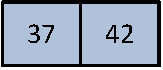
\includegraphics[height=0.5in]{figures/pair.pdf}
\end{centernospace}

Scheme provides built-in procedures for constructing a Pair, and for extracting each cell from a Pair:\index{general}{cons}\index{general}{car}\index{general}{cdr}

\begin{descriptionlist}
\item[\scheme|cons|: Value $\times$ Value $\rightarrow$ Pair] \forcenl Evaluates to a Pair whose first cell is the first input and second cell is the second input.  The inputs can be of any type.
\item[\scheme|car|: Pair $\rightarrow$ Value] \forcenl Evaluates to the first cell of the input, which must be a Pair.
\item[\scheme|cdr|: Pair $\rightarrow$ Value] \forcenl Evaluates to the second cell of input, which must be a Pair.
\end{descriptionlist}

These rather unfortunate names come from the original LISP implementation on the IBM 704.  The name \scheme|cons| is short for ``construct''.  The name \scheme|car| is short for ``\emph{C}ontents of the \emph{A}ddress part of the \emph{R}egister'' and the name \scheme|cdr| (pronounced ``could-er'') is short for ``\emph{C}ontents of the \emph{D}ecrement part of the \emph{R}egister''.  The designers of the original LISP implementation picked the names because of how pairs could be implemented on the IBM 704 using a single register to store both parts of a pair, but it is a mistake to name things after details of their implementation (see Section~\ref{sec:dataabstraction}).  Unfortunately, the names stuck.% and continue to be used.% in many LISP-derived languages, including Scheme.
  
We can construct the Pair shown above by evaluating \scheme|(cons 37 42)|.  DrRacket displays a Pair by printing the value of each cell separated by a dot: \schemeresult|(37 . 42)|.  The interactions below show example uses of \scheme|cons|, \scheme|car|, and \scheme|cdr|.

\begin{code}
\scheme|> (define mypair (cons 37 42))|\\
%\scheme|> mypair|\\
%\schemeresult|(37 . 42)|\\
\scheme|> (car mypair)|\\
\schemeresult|37|\\
\scheme|> (cdr mypair)|\\
\schemeresult|42|
\end{code}

The values in the cells of a Pair can be any type, including other Pairs.  For example, this definition defines a Pair where each cell of the Pair is itself a Pair:
\begin{schemedisplay}
(define doublepair (cons (cons 1 2) (cons 3 4)))
\end{schemedisplay}

We can use the \scheme|car| and \scheme|cdr| procedures to access components of the \scheme|doublepair| structure: \scheme|(car doublepair)| evaluates to the Pair \schemeresult|(1 . 2)|, and \scheme|(cdr doublepair)| evaluates to the Pair \schemeresult|(3 . 4)|.

We can compose multiple \scheme|car| and \scheme|cdr| applications to extract components from nested pairs:

\begin{code}
\scheme|> (cdr (car doublepair))|\\
\schemeresult|2|\\
\scheme|> (car (cdr doublepair))|\\
\schemeresult|3|\\
\scheme|> ((fcompose cdr cdr) doublepair)|\begin{scaside}\scheme|fcompose| from Section~4.2.1\end{scaside}\\ %%\ref{sec:fcompose}
\schemeresult|4|\\
\scheme|> (car (car (car doublepair)))|\\
\bugresult{car: expects argument of type $<$pair$>$; given 1}
\end{code}

The last expression produces an error when it is evaluated since \scheme|car| is applied to the scalar value \scheme|1|.  The \scheme|car| and \scheme|cdr| procedures can only be applied to an input that is a Pair.  Hence, an error results when we attempt to apply \scheme|car| to a scalar value.  This is an important property of data: the type of data (e.g., a Pair) defines how it can be used (e.g., passed as the input to \scheme|car| and \scheme|cdr|).  Every procedure expects a certain type of inputs, and typically produces an error when it is applied to values of the wrong type.

We can draw the value of \scheme|doublepair| by nesting Pairs within cells:
\begin{centernospace}
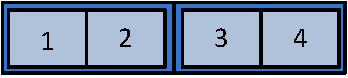
\includegraphics[width=2.0in]{figures/doublepair.pdf}
\end{centernospace}

Drawing Pairs within Pairs within Pairs can get quite difficult, however.  For instance, try drawing \scheme|(cons 1 (cons 2 (cons 3 (cons 4 5))))| this way.

Instead, we us arrows to point to the contents of cells that are not simple values.  This is the structure of \scheme|doublepair| shown using arrows:
\begin{centernospace}
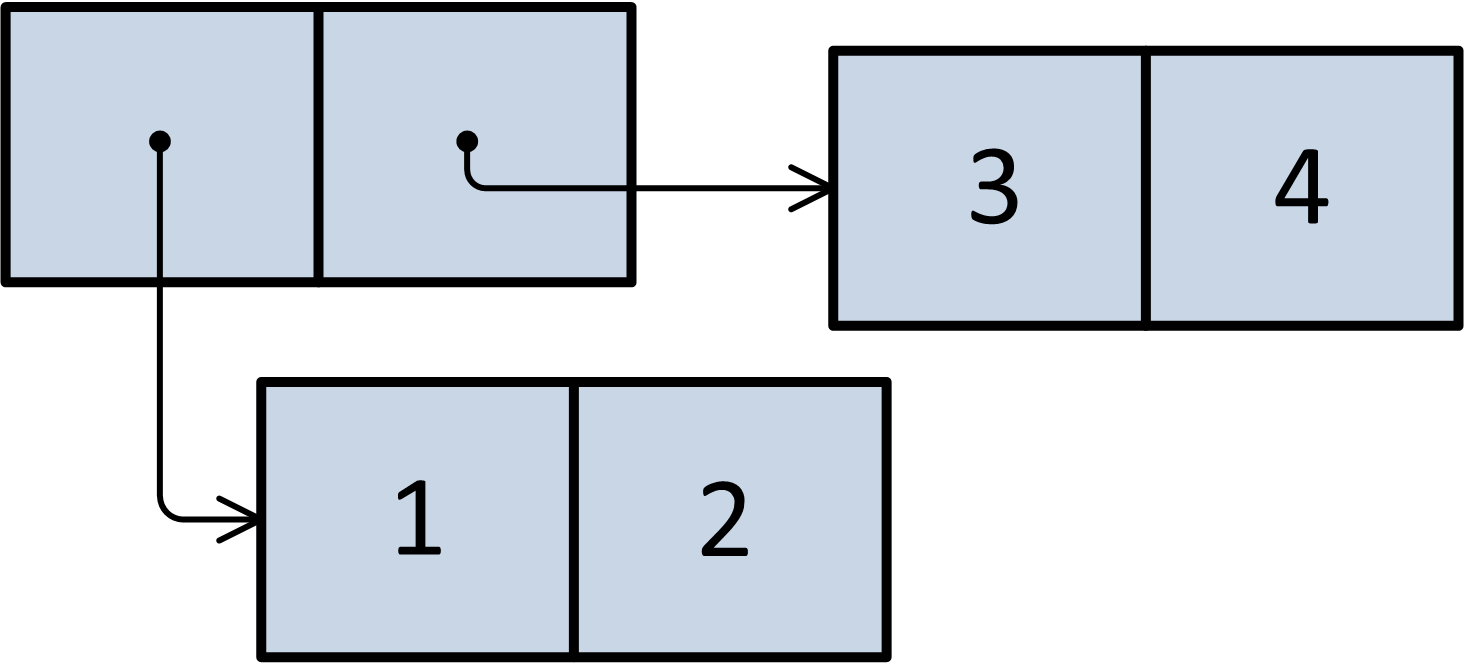
\includegraphics[width=2.0in]{figures/doublepair-arrows.png}
\end{centernospace}

Using arrows to point to cell contents allows us to draw arbitrarily complicated data structures such as \scheme|(cons 1 (cons 2 (cons 3 (cons 4 5))))|, keeping the cells reasonable sizes:
\begin{centernospace}
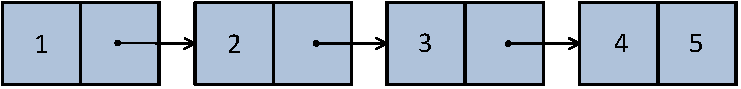
\includegraphics[width=3.5in]{figures/cons12345.pdf}
\end{centernospace}

\beforeex
\begin{exercise}
Suppose the following definition has been executed:
\begin{schemedisplay}
(define tpair 
  (cons (cons (cons 1 2) (cons 3 4)) 
        5))
\end{schemedisplay}
Draw the structure defined by \scheme|tpair|, and give the value of each of the following expressions.
% evaluates to (try evaluating each expression in a Scheme interpreter to check your answers).  
\begin{subexerciselist}
\item \scheme|(cdr tpair)|
\solution{\LATER{}}
\item \scheme|(car (car (car tpair)))|
\solution{\LATER{}}
\item \scheme|(cdr (cdr (car tpair)))|
\solution{\LATER{}}
\item \scheme|(car (cdr (cdr tpair)))|
\solution{\LATER{}}
\end{subexerciselist}
\end{exercise}
\afterex

\beforeex
\begin{exercise}
Write expressions that extract each of the four elements from \scheme|fstruct| defined by \scheme|(define fstruct (cons 1 (cons 2 (cons 3 4))))|.
\solution{\LATER{}}
\end{exercise}
\afterex

\beforeex
\begin{exercise}
Give an expression that produces the structure shown below.
\begin{center}
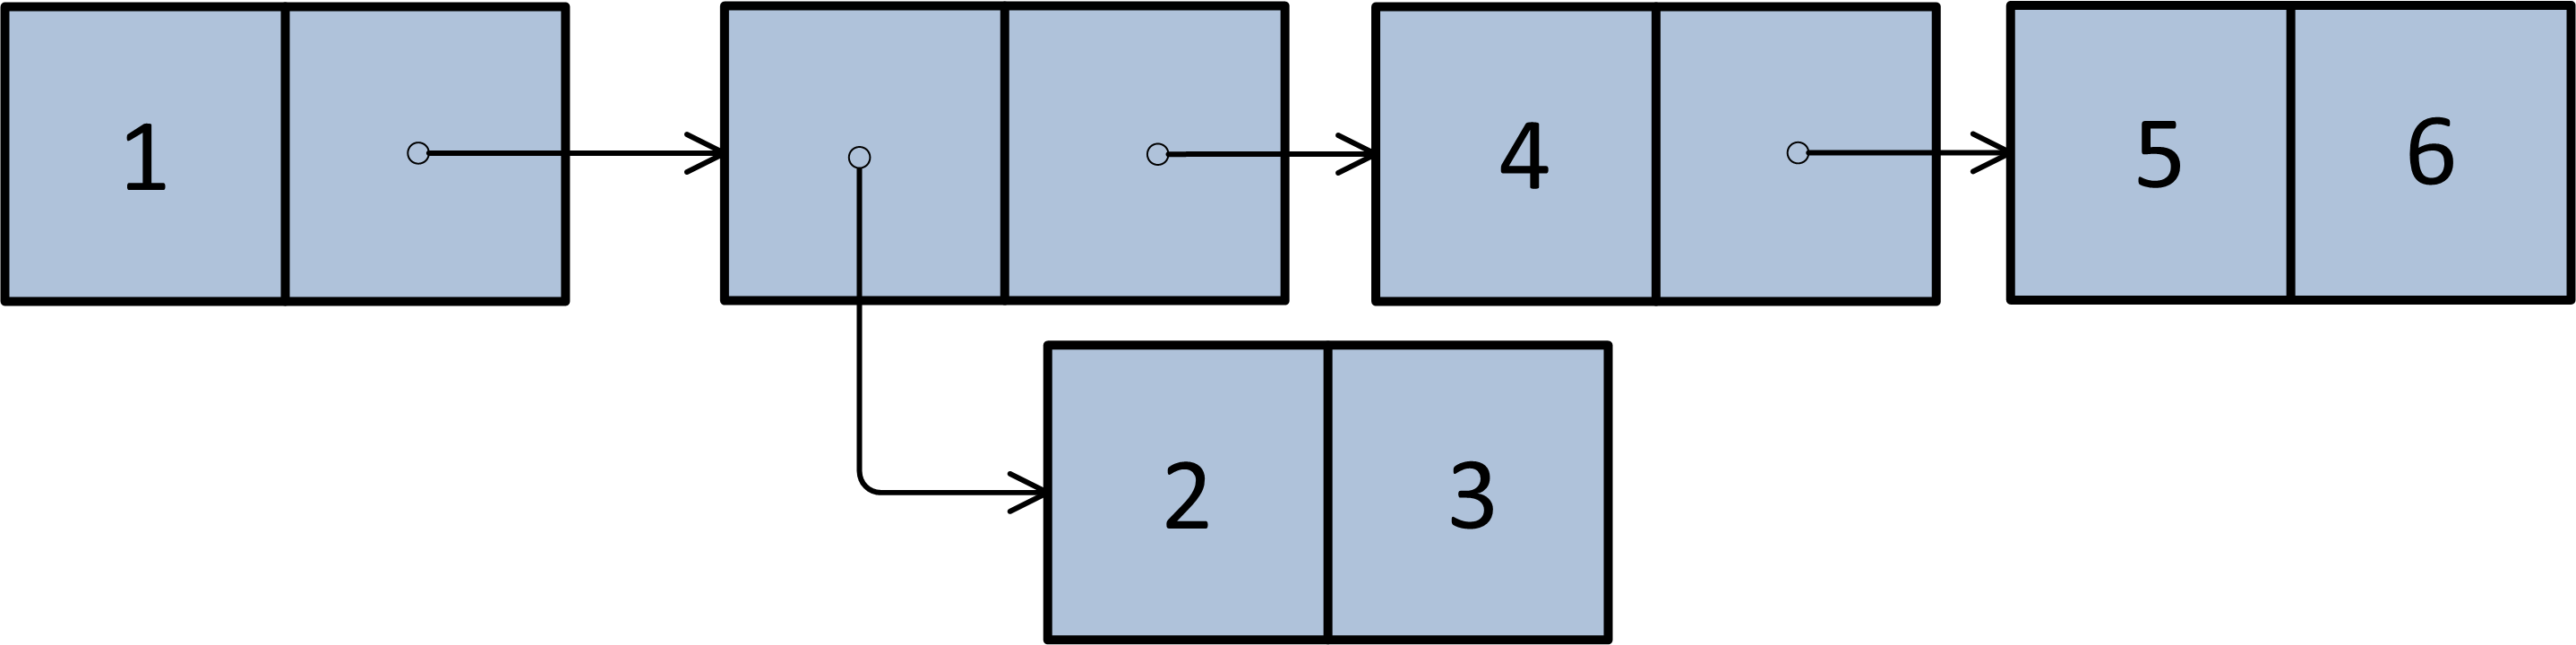
\includegraphics[width=3.5in]{figures/exstruct.png} 
\end{center}
\solution{\LATER{}}
\end{exercise}
\afterex

\subsection{Making Pairs}\label{sec:makingpairs}

Although Scheme provides the built-in procedures \scheme|cons|, \scheme|car|, and \scheme|cdr| for creating Pairs and accessing their cells, there is nothing magical about these procedures.  We can define procedures with the same behavior ourselves using the subset of Scheme introduced in Chapter~\ref{ch:programming}.  

Here is one way to define the pair procedures (we prepend an \emph{s} to the names to avoid confusion with the built-in procedures):
\begin{schemedisplay}
(define (scons a b) (lambda (w) (if w a b)))
(define (scar pair) (pair true))
(define (scdr pair) (pair false))
\end{schemedisplay}
The \scheme|scons| procedure takes the two parts of the Pair as inputs, and produces as output a procedure.  The output procedure takes one input, a selector that determines which of the two cells of the Pair to output.  If the selector is true, the value of the if expression is the value of the first cell; if the selector is false, it is the value of the second cell.  The \scheme|scar| and \scheme|scdr| procedures apply a procedure constructed by \scheme|scons| to either \scheme|true| (to select the first cell in \scheme|scar|) or \scheme|false| (to select the second cell in \scheme|scdr|).

\beforeex
\begin{exercise}
Convince yourself the definitions of \scheme|scons|, \scheme|scar|, and \scheme|scdr| above work as expected by following the evaluation rules to evaluate 
\begin{schemedisplay}
(scar (scons 1 2))
\end{schemedisplay}
\solution{\LATER{}}
\end{exercise}
\afterex

\beforeex
\begin{exercise}
Show the corresponding definitions of \scheme|tcar| and \scheme|tcdr| that provide the pair selection behavior for a pair created using \scheme|tcons| defined as:
\begin{schemedisplay}
(define (tcons a b) (lambda (w) (if w b a)))
\end{schemedisplay}
\solution{\LATER{}}
\end{exercise}
\afterex

\index{general}{Pair|)}

\subsection{Triples to Octuples}

Pairs are useful for representing data that is composed of two parts such as a calendar date (composed of a number and month), or a playing card (composed of a rank and suit).  But, what if we want to represent data composed of more than two parts such as a date (composed of a number, month, and year) or a poker hand consisting of five playing cards?   For more complex data structures, we need data structures that have more than two components.

A \emph{triple} has three components.  Here is one way to define a triple datatype:
\begin{schemedisplay}
(define (make-triple a b c) 
  (lambda (w) (if (= w 0) a (if (= w 1) b c))))                
(define (triple-first t)  (t 0))
(define (triple-second t) (t 1))
(define (triple-third t)  (t 2))
\end{schemedisplay}

Since a triple has three components we need three different selector values.  %We use \scheme|0|, \scheme|1|, and \scheme|2|.

Another way to make a triple would be to combine two Pairs.  We do this by making a Pair whose second cell is itself a Pair:
\begin{schemedisplay}
(define (make-triple a b c) (cons a (cons b c)))
(define (triple-first t)  (car t))
(define (triple-second t) (car (cdr t)))
(define (triple-third t)  (cdr (cdr t)))
\end{schemedisplay}

Similarly, we can define a \emph{quadruple} as a Pair whose second cell is a triple:
\begin{schemedisplay}
(define (make-quad a b c d) (cons a (make-triple b c d)))
(define (quad-first q)  (car q))
(define (quad-second q) (triple-first (cdr q))
(define (quad-third q)  (triple-second (cdr q))
(define (quad-fourth q) (triple-third (cdr q))
\end{schemedisplay}

We could continue in this manner defining increasingly large tuples.  
\begin{tightdescriptionlist}
\item[A \emph{triple} is a Pair whose second cell is a Pair.]
\item[A \emph{quadruple} is a Pair whose second cell is a \emph{triple}.]
\item[A \emph{quintuple} is a Pair whose second cell is a \emph{quadruple}.]
%\item[A \emph{sextuple} is a Pair whose second cell is a \emph{quintuple}.]
%\item[A \emph{septuple} is a Pair whose second cell is a \emph{sextuple}.]
\item[$\cdots$]
\item[An $n+1$\emph{-uple} is a Pair whose second cell is an \emph{n-uple}.]
\end{tightdescriptionlist}
Building from the simple Pair, we can construct tuples containing any number of components.

\beforeex
\begin{exercise}
Define a procedure that constructs a quintuple and procedures for selecting the five elements of a quintuple.
\solution{\LATER{}}
\end{exercise}
\afterex

\beforeex
\begin{exercise}
Another way of thinking of a triple is as a Pair where the first cell is a Pair and the second cell is a scalar.  Provide definitions of \scheme|make-triple|, \scheme|triple-first|, \scheme|triple-second|, and \scheme|triple-third| for this construct.
\solution{\LATER{}}
\end{exercise}
\afterex

\section{Lists}\label{sec:list}\index{general}{list|(}
In the previous section, we saw how to construct arbitrarily large tuples from Pairs.  This way of managing data is not very satisfying since it requires defining different procedures for constructing and accessing elements of every length tuple.  For many applications, we want to be able to manage data of any length such as all the items in a web store, or all the bids on a given item.  Since the number of components in these objects can change, it would be very painful to need to define a new tuple type every time an item is added.  We need a data type that can hold \emph{any} number of items.  

%What we want is a way to construct and manipulate tuples that works for tuples containing \emph{any} number of elements. 
This definition almost provides what we need: \index{general}{any-uple}
\begin{smallquote}
An \emph{any-uple} is a Pair whose second cell is an \emph{any-uple}.
\end{smallquote}

This seems to allow an \emph{any-uple} to contain any number of elements.  The problem is we have no stopping point.  With only the definition above, there is no way to construct an \emph{any-uple} without already having one.  

The situation is similar to defining \nonterminal{MoreDigits} as zero or more digits in Chapter~\ref{ch:language}, defining \nonterminal{MoreExpressions} in the Scheme grammar in Chapter~\ref{ch:programming} as zero or more \nonterminal{Expression}s, and recursive composition in Chapter~\ref{ch:problems}. 

Recall the grammar rules for \nonterminal{MoreExpressions}:
\begin{bnfgrammarm}{MoreExpressions}
\bnfrule{MoreExpressions}{\nonterminal{Expression} \nonterminal{MoreExpressions}}
\bnfrule{MoreExpressions}{$\epsilon$}
\end{bnfgrammarm}
The rule for constructing an \emph{any-uple} is analogous to the first \nonterminal{MoreExpression} replacement rule.  To allow an \emph{any-uple} to be constructed, we also need a construction rule similar to the second rule, where \nonterminal{MoreExpression} can be replaced with nothing.  Since it is hard to type and read nothing in a program, Scheme has a name for this value: \definition{null}.  

DrRacket will print out the value of \scheme|null| as \schemeresult|()|.  It is also known as the \emph{empty list}, since it represents the List containing no elements.  The built-in procedure \scheme|null?| takes one input parameter and evaluates to \schemeresult|true| if and only if the value of that parameter is \schemeresult|null|.\index{general}{null?}

Using \schemeresult|null|, we can now define a \indexeddefinition{List}{list}: 
\begin{smallquote}
A \emph{List} is either (1) \schemeresult{null} or (2) a Pair whose second cell is a \emph{List}.
\end{smallquote}

Symbolically, we define a List as:
\begin{bnfgrammarm}{Listx}
\bnfrule{List}{\schemeresult|null|}
\bnfrule{List}{\scheme|(cons \value \List)|}
\end{bnfgrammarm}

These two rules define a List as a data structure that can contain any number of elements.  Starting from \schemeresult|null|, we can create Lists of any length:
\begin{itemtight}
\item \scheme|null| evaluates to a List containing no elements.
\item \scheme|(cons 1 null)| evaluates to a List containing one element.
\item \scheme|(cons 1 (cons 2 null))| evaluates to a List containing two elements.
\item \scheme|(cons 1 (cons 2 (cons 3 null)))| evaluates to a 3-element List.
%\item $\ldots$
\end{itemtight}

Scheme provides a convenient procedure, \scheme|list|, for constructing a List.  The \scheme|list| procedure takes zero or more inputs, and evaluates to a List containing those inputs in order.  The following expressions are equivalent to the corresponding expressions above: \scheme|(list)|, \scheme|(list 1)|, \scheme|(list 1 2)|, and \scheme|(list 1 2 3)|.

Lists are just a collection of Pairs, so we can draw a List using the same box and arrow notation we used to draw structures created with Pairs.  Here is the structure resulting from \scheme|(list 1 2 3)|:  
\begin{center}
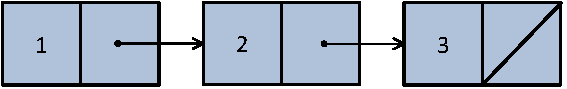
\includegraphics[width=3.5in]{figures/list.pdf}
\end{center}
There are three Pairs in the List, the second cell of each Pair is a List.  For the third Pair, the second cell is the List \scheme|null|, which we draw as a slash through the final cell in the diagram.

Table~\ref{tab:list-procs} summarizes some of the built-in procedures for manipulating Pairs and Lists.
%\begin{center}
\begin{table}[b]
\small \raggedright
\begin{tabular}{cp{1.7in}p{2.5in}} %\hline
\multicolumn{1}{c}{} & \multicolumn{1}{c}{\bfseries Type} & \multicolumn{1}{c}{\bfseries Output} \tabularnewline[6pt] 
\scheme|cons|  & \raggedright Value $\times$ Value $\rightarrow$ Pair & \raggedright	a Pair consisting of the two inputs\tabularnewline[3pt]  
\scheme|car|   & \raggedright Pair $\rightarrow$ Value & \raggedright the first cell of the input Pair \tabularnewline[3pt]
\scheme|cdr|	 & \raggedright Pair $\rightarrow$ Value & \raggedright the second cell of the input Pair \tabularnewline[3pt] 
\scheme|list|  & \raggedright zero or more Values $\rightarrow$ List & \raggedright a List containing the inputs \tabularnewline[3pt] % \hline
\scheme|null?|  & \raggedright Value $\rightarrow$ Boolean & \raggedright \schemeresult|true| if the input is \schemeresult|null|, otherwise \schemeresult|false| \tabularnewline[3pt] % \hline
\scheme|pair?|  & \raggedright Value $\rightarrow$ Boolean & \raggedright \schemeresult|true| if the input is a Pair, otherwise \schemeresult|false|\tabularnewline[3pt] % \hline
\scheme|list?|  & \raggedright Value $\rightarrow$ Boolean & \raggedright \schemeresult|true| if the input is a List, otherwise \schemeresult|false|\tabularnewline[6pt] % \hline
\end{tabular} \\[0.5ex]
\caption{\label{tab:list-procs} Selected Built-In Scheme Procedures for Lists and Pairs.} \index{general}{list procedures}
\vspace{0.5cm}
\end{table}
%\end{center}

\beforesplitex
\begin{exercise}\label{ex:lists}
For each of the following expressions, explain whether or not the expression evaluates to a List.  Check your answers with a Scheme interpreter by using the \scheme|list?| procedure.
\begin{subexerciselist}
\item \scheme|null|
\item \scheme|(cons 1 2)|
%\item \scheme|(cons 1 null)|
\item \scheme|(cons null null)|
\item \scheme|(cons (cons (cons 1 2) 3) null)|
%\item \scheme|(cons 1 (cons 2 (cons 3 (cons 4 null))))|
\item \scheme|(cdr (cons 1 (cons 2 (cons null null))))|
\item \scheme|(cons (list 1 2 3) 4)|
\end{subexerciselist}
\solution{\LATER{}}
\end{exercise}
\aftersplitex

\index{general}{list|)}

\section{List Procedures}\label{sec:listprocedures}

Since the List data structure is defined recursively, it is natural to define recursive procedures to examine and manipulate lists.  Whereas most recursive procedures on inputs that are Numbers usually used \scheme|0| as the base case, for lists the most common base case is \scheme|null|.  With numbers, we make progress by subtracting \scheme|1|; with lists, we make progress by using \scheme|cdr| to reduce the length of the input List by one element for each recursive application.  This means we often break problems involving Lists into figuring out what to do with the first element of the List and the result of applying the recursive procedure to the rest of the List.  

We can specialize our general problem solving strategy from Chapter~\ref{ch:programming} for procedures involving lists:
\begin{enumerate}
\item \bold{Be \emph{very} optimistic!}  Since lists themselves are recursive data structures, most problems involving lists can be solved with recursive procedures.
\item Think of the simplest version of the problem, something you can already solve.  This is the base case.  For lists, this is usually the empty list.
\item Consider how you would solve a big version of the problem by using the result for a slightly smaller version of the problem.  This is the recursive case.  For lists, the smaller version of the problem is usually the rest (\scheme|cdr|) of the List.
\item Combine the base case and the recursive case to solve the problem.
\end{enumerate}

Next we consider procedures that examine lists by walking through their elements and producing a scalar value.  Section~\ref{sec:generic} generalizes these procedures.  In Section~\ref{sec:constructing-lists}, we explore procedures that output lists.

\subsection{Procedures that Examine Lists}\label{sec:examining-lists}

All of the example procedures in this section take a single List as input and produce a scalar value that depends on the elements of the List as output.  These procedures have base cases where the List is empty, and recursive cases that apply the recursive procedure to the \scheme|cdr| of the input List.

%%\clearpage %%!
\begin{examplenobar}{Length}\label{example:length}\index{general}{length}\index{general}{list-length}  How many elements are in a given List?\footnote{Scheme provides a built-in procedure \scheme|length| that takes a List as its input and outputs the number of elements in the List.  Here, we will define our own \scheme|list-length| procedure that does this (without using the built-in \scheme|length| procedure).  As with many other examples and exercises in this chapter, it is instructive to define our own versions of some of the built-in list procedures.}  Our standard recursive problem solving technique is to ``Think of the simplest version of the problem, something you can already solve.''  For this procedure, the simplest version of the problem is when the input is the empty list, \scheme|null|.  We know the length of the empty list is \schemeresult|0|.  So, the base case test is \scheme|(null? p)| and the output for the base case is \scheme|0|.

For the recursive case, we need to consider the structure of all lists other than \scheme|null|.  Recall from our definition that a List is either \scheme|null| or \scheme|(cons \value \List)|.  The base case handles the \scheme|null| list; the recursive case must handle a List that is a Pair of an element and a List.  The length of this List is one more than the length of the List that is the \scheme|cdr| of the Pair.

\begin{schemedisplay}
(define (list-length p)
   (if (null? p) 
       0 
       (+ 1 (list-length (cdr p)))))
\end{schemedisplay}

Here are a few example applications of our \scheme|list-length| procedure:
\begin{code}
\scheme|> (list-length null)|\\
\schemeresult|0|\\
\scheme|> (list-length (cons 0 null))|\\
\schemeresult|1|\\
\scheme|> (list-length (list 1 2 3 4))|\\
\schemeresult|4|%\\
%\scheme|> (list-length (cons 1 2))|\begin{aside}Error since input is not a List.\end{aside}
%\bugresult{cdr: expects argument of type $<$pair$>$; given 2}\\
\end{code}
\end{examplenobar}

\begin{examplenobar}{List Sums and Products}\label{example:list-sum} First, we define a procedure that takes a List of numbers as input and produces as output the sum of the numbers in the input List.  As usual, the base case is when the input is \scheme|null|: the sum of an empty list is \scheme|0|.  For the recursive case, we need to add the value of the first number in the List, to the sum of the rest of the numbers in the List.  \index{general}{list-sum}
\begin{schemedisplay}
(define (list-sum p)
   (if (null? p) 0 (+ (car p) (list-sum (cdr p)))))
\end{schemedisplay}
We can define \scheme{list-product} similarly, using \scheme|*| in place of \scheme|+|.  The base case result cannot be \scheme|0|, though, since then the final result would always be \schemeresult|0| since any number multiplied by \scheme|0| is \scheme|0|.  We follow the mathematical convention that the product of the empty list is \scheme|1|.\index{general}{list-product}
\begin{schemedisplay}
(define (list-product p)
   (if (null? p) 1 (* (car p) (list-product (cdr p)))))
\end{schemedisplay}
\end{examplenobar}

\beforeex
\begin{exercise}\label{ex:listq} \bluestar
Define a procedure \scheme|is-list?| that takes one input and outputs \schemeresult{true} if the input is a List, and \schemeresult{false} otherwise.  Your procedure should behave identically to the built-in \scheme|list?| procedure, but you should not use \scheme|list?| in your definition.  %Hint: recall the definition of a List in Section~\ref{sec:list}.
\solution{\LATER{}}
\end{exercise}
\afterex

\beforeex
\begin{exercise}\label{ex:list-max} \greenstar
Define a procedure \scheme|list-max| that takes a List of non-negative numbers as its input and produces as its result the value of the greatest element in the List (or \schemeresult|0| if there are no elements in the input List).  For example, \scheme|(list-max (list 1 1 2 0))| should evaluate to \schemeresult|2|.
\solution{\LATER{}}
\end{exercise}
\afterex

\subsection{Generic Accumulators}\label{sec:generic}\index{general}{accumulators}

The \scheme|list-length|, \scheme|list-sum|, and \scheme|list-product| procedures all have very similar structures.  The base case is when the input is the empty list, and the recursive case involves doing something with the first element of the List and recursively calling the procedure with the rest of the List:

\begin{schemedisplay}
(define (\recproc p)
   (if (null? p)
       \basecaseres
       (\accumfunc (car p) (\recproc (cdr p)))))
\end{schemedisplay}

We can define a generic accumulator procedure for lists by making the base case result and accumulator function inputs:
\begin{schemedisplay}
(define (list-accumulate f base p)
  (if (null? p) 
      base
      (f (car p) (list-accumulate f base (cdr p)))))
\end{schemedisplay}

We can use \scheme|list-accumulate| to define \scheme|list-sum| and \scheme|list-product|:
\begin{schemedisplay}
(define (list-sum p) (list-accumulate + 0 p))
(define (list-product p) (list-accumulate * 1 p))
\end{schemedisplay}

Defining the \scheme|list-length| procedure is a bit less natural.  The recursive case in the original \scheme|list-length| procedure is \scheme|(+ 1 (list-length (cdr p)))|; it does not use the value of the first element of the List.  But, \scheme|list-accumulate| is defined to take a procedure that takes two inputs---the first input is the first element of the List; the second input is the result of applying \scheme|list-accumulate| to the rest of the List.  We should follow our usual strategy: be optimistic!  Being optimistic as in recursive definitions, the value of the second input should be the length of the rest of the List.  Hence, we need to pass in a procedure that takes two inputs, ignores the first input, and outputs one more than the value of the second input:
\begin{schemedisplay}
(define (list-length p) 
  (list-accumulate (lambda (el length-rest) (+ 1 length-rest)) 0 p))
\end{schemedisplay}

\beforeex
\begin{exercise}
Use \scheme|list-accumulate| to define \scheme|list-max| (from Exercise~\ref{ex:list-max}).
\solution{\LATER{}}
\end{exercise}
\afterex

\beforeex
\begin{exercise}
\goldstar Use \scheme|list-accumulate| to define \scheme|is-list?| (from Exercise~\ref{ex:listq}).
\solution{\LATER{}}
\end{exercise}
\afterex

%%\clearpage %!!
\begin{examplenobar}{Accessing List Elements}\label{example:list-get-element}\index{general}{list-get-element}
The built-in \scheme|car| procedure provides a way to get the first element of a list, but what if we want to get the third element?  We can do this by taking the \scheme|cdr| twice to eliminate the first two elements, and then using \scheme|car| to get the third: 
\begin{schemedisplay}
(car (cdr (cdr p)))
\end{schemedisplay}

We want a more general procedure that can access any selected list element.  It takes two inputs: a List, and an index Number that identifies the element.  If we start counting from \scheme|1| (it is often more natural to start from \scheme|0|), then the base case is when the index is \scheme|1| and the output should be the first element of the List: 
\begin{schemedisplay}
(if (= n 1) (car p) \rest)
\end{schemedisplay}

For the recursive case, we make progress by eliminating the first element of the list.  We also need to adjust the index: since we have removed the first element of the list, the index should be reduced by one.  For example, instead of wanting the third element of the original list, we now want the second element of the \scheme|cdr| of the original list.

\begin{schemedisplay}
(define (list-get-element p n) 
   (if (= n 1)
       (car p)
       (list-get-element (cdr p) (- n 1))))
\end{schemedisplay}

What happens if we apply \scheme|list-get-element| to an index that is larger than the size of the input List (for example, \scheme|(list-get-element (list 1 2) 3)|)?

The first recursive call is \scheme|(list-get-element (list 2) 2)|.  The second recursive call is \scheme|(list-get-element (list) 1)|.  At this point, \scheme|n| is \scheme|1|, so the base case is reached and \scheme|(car p)| is evaluated.  But, \scheme|p| is the empty list (which is not a Pair), so an error results.

A better version of \scheme|list-get-element| would provide a meaningful error message when the requested element is out of range.  We do this by adding an if expression that tests if the input List is \scheme|null|:
\begin{schemedisplay}
(define (list-get-element p n) 
   (if (null? p)
       (error "Index out of range")
       (if (= n 1) (car p) (list-get-element (cdr p) (- n 1)))))
\end{schemedisplay}
The built-in procedure \scheme|error| takes a String as input.  The String datatype is a sequence of characters; we can create a String by surrounding characters with double quotes, as in the example.  The \scheme|error| procedure terminates program execution with a message that displays the input value.

Checking explicitly for invalid inputs is known as \definition{defensive programming}.  Programming defensively helps avoid tricky to debug errors and makes it easier to understand what went wrong if there is an error.

\end{examplenobar}

\beforeex
\begin{exercise}
\bluestar Define a procedure \scheme|list-last-element| that takes as input a List and outputs the last element of the input List.  If the input List is empty, \scheme|list-last-element| should produce an error.
\solution{\LATER{}}
\end{exercise}
\afterex

\beforeex
\begin{exercise}
\greenstar
Define a procedure \scheme{list-ordered?} that takes two inputs, a test procedure and a List.  It outputs true if all the elements of the List are ordered according to the test procedure.  For example, \scheme{(list-ordered? < (list 1 2 3))} evaluates to \schemeresult{true}, and \scheme{(list-ordered? < (list 1 2 3 2))} evaluates to \schemeresult{false}.  Hint: think about what the output should be for the empty list.
\solution{\LATER{}}
\end{exercise}
\afterex

\subsection{Procedures that Construct Lists}\label{sec:constructing-lists}

The procedures in this section take values (including Lists) as input, and produce a new List as output.  As before, the empty list is typically the base case.  Since we are producing a List as output, the result for the base case is also usually \schemeresult|null|.  The recursive case will use \scheme|cons| to construct a List combining the first element with the result of the recursive application on the rest of the List.

\begin{examplenobar}{Mapping}\label{example:map}\index{general}{list-map}\index{general}{map} One common task for manipulating a List is to produce a new List that is the result of applying some procedure to every element in the input List.  

For the base case, applying any procedure to every element of the empty list produces the empty list.  For the recursive case, we use \scheme|cons| to construct a List.  The first element is the result of applying the mapping procedure to the first element of the input List.  The rest of the output List is the result of recursively mapping the rest of the input List.

Here is a procedure that constructs a List that contains the square of every element of the input List:

\begin{schemedisplay}
(define (list-square p)
  (if (null? p) null
      (cons (square (car p)) 
            (list-square (cdr p)))))
\end{schemedisplay}

We generalize this by making the procedure which is applied to each element an input.  The procedure \scheme|list-map| takes a procedure as its first input and a List as its second input.  It outputs a List whose elements are the results of applying the input procedure to each element of the input List.\footnote{Scheme provides a built-in \scheme|map| procedure.  It behaves like this one when passed a procedure and a single List as inputs, but can also work on more than one List input at a time.}

\begin{schemedisplay}
(define (list-map f p)
  (if (null? p) null
      (cons (f (car p)) 
            (list-map f (cdr p)))))
\end{schemedisplay}

We can use \scheme|list-map| to define \scheme|square-all|:
\begin{schemedisplay}
(define (square-all p) (list-map square p))
\end{schemedisplay}

\beforeex
\begin{exercise}
Define a procedure \scheme|list-increment| that takes as input a List of numbers, and produces as output a List containing each element in the input List incremented by one.  For example, \scheme|(list-increment 1 2 3)| evaluates to \schemeresult|(2 3 4)|.
\solution{\LATER{}}
\end{exercise}
\afterex

\beforeex
\begin{exercise}
Use \scheme|list-map| and \scheme|list-sum| to define \scheme|list-length|: 
\begin{schemedisplay}
(define (list-length p) (list-sum (list-map \fillspace p)))
\end{schemedisplay}
\solution{\LATER{}}
\end{exercise}
\afterex

\end{examplenobar}

\begin{examplenobar}{Filtering}\label{example:filter}\index{general}{filtering}  Consider defining a procedure that takes as input a List of numbers, and evaluates to a List of all the non-negative numbers in the input.  For example, \scheme|(list-filter-negative (list 1 -3 -4 5 -2 0))| evaluates to \schemeresult|(1 5 0)|.

First, consider the base case when the input is the empty list.  If we filter the negative numbers from the empty list, the result is an empty list.  So, for the base case, the result should be \schemeresult|null|.  

In the recursive case, we need to determine whether or not the first element should be included in the output.  If it should be included, we construct a new List consisting of the first element followed by the result of filtering the remaining elements in the List.  If it should not be included, we skip the first element and the result is the result of filtering the remaining elements in the List.

\begin{schemedisplay}
(define (list-filter-negative p)
  (if (null? p) null
      (if (>= (car p) 0)
          (cons (car p) (list-filter-negative (cdr p)))
          (list-filter-negative (cdr p)))))
\end{schemedisplay}

Similarly to \scheme|list-map|, we can generalize our filter by making the test procedure as an input, so we can use any predicate to determine which elements to include in the output List.\footnote{Scheme provides a built-in function \scheme|filter| that behaves like our \scheme|list-filter| procedure.}

\begin{schemedisplay}
(define (list-filter test p)
  (if (null? p) null
      (if (test (car p))
          (cons (car p) (list-filter test (cdr p)))
          (list-filter test (cdr p)))))
\end{schemedisplay}

Using the \scheme|list-filter| procedure, we can define \scheme|list-filter-negative| as:
\begin{schemedisplay}
(define (list-filter-negative p) (list-filter (lambda (x) (>= x 0)) p))
\end{schemedisplay}

We could also define the \scheme|list-filter| procedure using the \scheme|list-accumulate| procedure from Section~\ref{sec:examining-lists}:
\begin{schemedisplay}
(define (list-filter test p)
  (list-accumulate 
    (lambda (el rest) (if (test el) (cons el rest) rest)) 
    null 
    p))
\end{schemedisplay}


\beforeex
\begin{exercise}
Define a procedure \scheme|list-filter-even| that takes as input a List of numbers and produces as output a List consisting of all the even elements of the input List.  
\solution{\LATER{}}
\end{exercise}
\afterex

\beforeex
\begin{exercise}\bluestar
Define a procedure \scheme|list-remove| that takes two inputs: a test procedure and a List.  As output, it produces a List that is a copy of the input List with all of the elements for which the test procedure evaluates to true removed.  For example, \scheme|(list-remove (lambda (x) (= x 0)) (list 0 1 2 3))| should evaluates to the List \schemeresult|(1 2 3)|.
\solution{\LATER{}}
\end{exercise}
\afterex

\beforeex
\begin{exercise}
\doublegoldstar
Define a procedure \scheme|list-unique-elements| that takes as input a List and produces as output a List containing the unique elements of the input List.  The output List should contain the elements in the same order as the input List, but should only contain the first appearance of each value in the input List.
\solution{\LATER{}}
\end{exercise}
\afterex

\end{examplenobar}

\begin{examplenobar}{Append}\label{example:append}\index{general}{append}\index{general}{list-append} The \scheme|list-append| procedure takes as input two lists and produces as output a List consisting of the elements of the first List followed by the elements of the second List.\footnote{There is a built-in procedure \scheme|append| that does this.  The built-in \scheme|append| takes any number of Lists as inputs, and appends them all into one List.}  For the base case, when the first List is empty, the result of appending the lists should just be the second List.  When the first List is non-empty, we can produce the result by \scheme|cons|-ing the first element of the first List with the result of appending the rest of the first List and the second List.
\begin{schemedisplay}
(define (list-append p q)
  (if (null? p) q
      (cons (car p) (list-append (cdr p) q))))
\end{schemedisplay}
\end{examplenobar}

\begin{examplenobar}{Reverse}\index{general}{reverse}\index{general}{list-reverse} The \scheme|list-reverse| procedure takes a List as input and produces as output a List containing the elements of the input List in reverse order.\footnote{The built-in procedure \scheme|reverse| does this.}  For example, \scheme|(list-reverse (list 1 2 3))| evaluates to the List \schemeresult|(3 2 1)|.  As usual, we consider the base case where the input List is \schemeresult|null| first.  The reverse of the empty list is the empty list.  To reverse a non-empty List, we should put the first element of the List at the end of the result of reversing the rest of the List.  

The tricky part is putting the first element at the end, since \scheme|cons| only puts elements at the beginning of a List.  We can use the \scheme|list-append| procedure defined in the previous example to put a List at the end of another List.  To make this work, we need to turn the element at the front of the List into a List containing just that element.  We do this using \scheme|(list (car p))|.

\begin{schemedisplay}
(define (list-reverse p)
  (if (null? p) null 
      (list-append (list-reverse (cdr p)) (list (car p)))))
\end{schemedisplay}

\begin{exercise} \greenstar
Define the \scheme|list-reverse| procedure using \scheme|list-accumulate|.
\end{exercise}

\end{examplenobar}

\begin{examplenobar}{Intsto}\label{example:intsto}\index{general}{intsto} For our final example, we define the \scheme|intsto| procedure that constructs a List containing the whole numbers between 1 and the input parameter value.  For example, \scheme|(intsto 5)| evaluates to the List \schemeresult|(1 2 3 4 5)|.  

This example combines ideas from the previous chapter on creating recursive definitions for problems involving numbers, and from this chapter on lists.  Since the input parameter is not a List, the base case is not the usual list base case when the input is \scheme|null|.  Instead, we use the input value \scheme|0| as the base case.  The result for input \scheme|0| is the empty list.  For higher values, the output is the result of putting the input value at the end of the List of numbers up to the input value minus one.

A first attempt that doesn't quite work is:
\begin{schemedisplay}
(define (revintsto n)
  (if (= n 0) null 
      (cons n (revintsto (- n 1)))))
\end{schemedisplay}
The problem with this solution is that it is \scheme|cons|-ing the higher number to the front of the result, instead of at the end.  Hence, it produces the List of numbers in descending order: \scheme|(revintsto 5)| evaluates to \schemeresult|(5 4 3 2 1)|.

One solution is to reverse the result by composing \scheme|list-reverse| with \scheme|revintsto|:
\begin{schemedisplay}
(define (intsto n) (list-reverse (revintsto n)))
\end{schemedisplay}
Equivalently, we can use the \scheme|fcompose| procedure from Section~\ref{sec:compose}:
\begin{schemedisplay}
(define intsto (fcompose list-reverse revintsto))
\end{schemedisplay}

Alternatively, we could use \scheme|list-append| to put the high number directly at the end of the List.  Since the second operand to \scheme|list-append| must be a List, we use \scheme|(list n)| to make a singleton List containing the value as we did for \scheme|list-reverse|.  
\begin{schemedisplay}
(define (intsto n)
  (if (= n 0) null 
      (list-append (intsto (- n 1)) (list n))))
\end{schemedisplay}
Although all of these procedures are functionally equivalent (for all valid inputs, each function produces exactly the same output), the amount of computing work (and hence the time they take to execute) varies across the implementations.  We consider the problem of estimating the running-times of different procedures in Part II.
\cut{We analyze the costs of evaluation in Chapter~\ref{ch:cost} and consider the costs of the different \scheme|intsto| implementations.\LATER{most specific reference}}

\beforeex
\begin{exercise}
Define \scheme|factorial| \cut{(from Example~\ref{ex:factorial}) }using \scheme|intsto|.\index{general}{factorial}
\solution{\LATER{}}
\end{exercise}
\afterex
\end{examplenobar}

\section{Lists of Lists}\label{sec:listsoflists}

The elements of a List can be any datatype, including, of course, other Lists.  In defining procedures that operate on Lists of Lists, we often use more than one recursive call when we need to go inside the inner Lists.  

\begin{examplenobar}{Summing Nested Lists}
Consider the problem of summing all the numbers in a List of Lists.  For example, \scheme|(nested-list-sum (list (list 1 2 3) (list 4 5 6)))| should evaluate to \schemeresult|21|.  We can define \scheme|nested-list-sum| using \scheme|list-sum| on each List.
\begin{schemedisplay}
(define (nested-list-sum p)
  (if (null? p) 0
      (+ (list-sum (car p))
         (nested-list-sum (cdr p)))))
\end{schemedisplay}
This works when we know the input is a List of Lists.  But, what if the input can contain arbitrarily deeply nested Lists?

To handle this, we need to recursively sum the inner Lists.  Each element in our deep List is either a List or a Number.  If it is a List, we should add the value of the sum of all elements in the List to the result for the rest of the List.  If it is a Number, we should just add the value of the Number to the result for the rest of the List.  So, our procedure involves two recursive calls: one for the first element in the List when it is a List, and the other for the rest of the List.
\begin{schemedisplay}
(define (deep-list-sum p)
  (if (null? p) 0
      (+ (if (list? (car p))
             (deep-list-sum (car p))
             (car p))
         (deep-list-sum (cdr p)))))
\end{schemedisplay}
\end{examplenobar}

\begin{examplenobar}{Flattening Lists}\label{example-list-flatten}\index{general}{flattening lists}\index{general}{list-flatten}
Another way to compute the deep list sum would be to first flatten the List, and then use the \scheme|list-sum| procedure.  

Flattening a nested list takes a List of Lists and evaluates to a List containing the elements of the inner Lists.  We can define \scheme|list-flatten| by using \scheme|list-append| to append all the inner Lists together.

\begin{schemedisplay}
(define (list-flatten p)
  (if (null? p) null
      (list-append (car p) (list-flatten (cdr p)))))
\end{schemedisplay}

This flattens a List of Lists into a single List.  To completely flatten a deeply nested List, we use multiple recursive calls as we did with \scheme|deep-list-sum|:
\begin{schemedisplay}
(define (deep-list-flatten p)
  (if (null? p) null
      (list-append (if (list? (car p))
                       (deep-list-flatten (car p))
                       (list (car p)))
                   (deep-list-flatten (cdr p)))))
\end{schemedisplay}
Now we can define \scheme|deep-list-sum| as: 
\begin{schemedisplay}
(define deep-list-sum (fcompose deep-list-flatten list-sum))
\end{schemedisplay}

\beforeex
\begin{exercise}\goldstar 
Define a procedure \scheme|deep-list-map| that behaves similarly to \scheme|list-map| but on deeply nested lists.  It should take two parameters, a mapping procedure, and a List (that may contain deeply nested Lists as elements), and output a List with the same structure as the input List with each value mapped using the mapping procedure.
\solution{\LATER{}}
\end{exercise}
\afterex

\beforeex
\begin{exercise} \goldstar 
Define a procedure \scheme|deep-list-filter| that behaves similarly to \scheme|list-filter| but on deeply nested lists.
\solution{\LATER{}}
\end{exercise}
\afterex

\end{examplenobar}

\splitexplorenobar{Pascal's Triangle}{\label{excur:pascal}\index{people}{Pascal, Blaise}\index{general}{Pascal's Triangle}

Pascal's Triangle (named for Blaise Pascal, although known to many others before him) is shown below: %in Figure~\ref{fig:pascalstriangle}.

%\begin{figure}[!htb]\centering
\begin{minipage}[b]{0.45\linewidth}\vspace{0pt}\centering{\sf
\begin{tabular}{@{}c@{}c@{}c@{}c@{}c@{}c@{}c@{}c@{}c@{}c@{}c@{}c@{}c}
 & & & & &1 & & & & & \\
 & & & &1 & &1 & & & & \\
 & & &1 & &2 & &1 & & & \\
 & & 1& &3 & &3 & &1& & \\
 & 1& &4 & &6 & &4 & &1& \\
 1& &5 & &10& &10& &5& &1\\
%1& &6 & &15& &20& &15& &6& & 1\\
 \multicolumn{10}{c}{$\cdots$} \\
 \end{tabular}\vspace*{12pt}}
\end{minipage}
\begin{minipage}[b]{0.4\linewidth}\vspace{0pt}
{\scalebox{0.2}{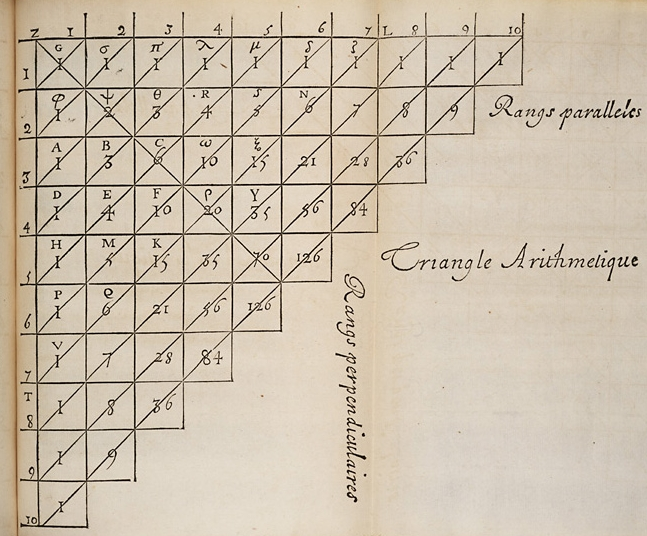
\includegraphics{images/pascaltriangle.jpg}}}%http://en.wikipedia.org/wiki/File:TrianguloPascal.jpg
\end{minipage}
%\caption{Pascal's Triangle}\label{fig:pascalstriangle}
%\end{figure}

Each number in the triangle is the sum of the two numbers immediately above and to the left and right of it.  The numbers in Pascal's Triangle are the coefficients in a binomial expansion.  The numbers of the $n^{th}$ row (where the rows are numbered starting from 0) are the coefficients of the binomial expansion of $(x+y)^n$.  For example, $(x+y)^2 = x^2+2xy+y^2$, so the coefficients are \scheme|1 2 1|, matching the third row in the triangle; from the fifth row, $(x+y)^4 = x^4 + 4x^3y + 6 x^2y^2 + 4xy^3 + y^4$.  The values in the triangle also match the number of ways to choose $k$ elements from a set of size $n$ (see Exercise~\ref{ex:nchoosek}) --- the $k^{th}$ number on the $n^{th}$ row of the triangle gives the number of ways to choose $k$ elements from a set of size $n$.  For example, the third number on the fifth ($n$ = 4) row is 6, so there are 6 ways to choose 3 items from a set of size 4.

\index{general}{binomial expansion}

The goal of this exploration is to define a procedure, \scheme|pascals-triangle| to produce Pascal's Triangle.  The input to your procedure should be the number of rows; the output should be a list, where each element of the list is a list of the numbers on that row of Pascal's Triangle.  For example, \scheme|(pascals-triangle 0)| should produce \schemeresult|((1))| (a list containing one element which is a list containing the number \schemeresult|1|), and \scheme|(pascals-triangle 4)| should produce \schemeresult|((1) (1 1) (1 2 1) (1 3 3 1) (1 4 6 4 1))|.

Ambitious readers should attempt to define \scheme|pascals-triangle| themselves; the sub-parts below provide some hints for one way to define it.
\begin{subexerciselist}
\item First, define a procedure \scheme|expand-row| that expands one row in the triangle.  It takes a List of numbers as input, and as output produces a List with one more element than the input list.  The first number in the output List should be the first number in the input List; the last number in the output List should be the last number in the input List.  Every other number in the output List is the sum of two numbers in the input List.  The $n^{th}$ number in the output List is the sum of the $n-1^{th}$ and $n^{th}$ numbers in the input List.  For example, \scheme|(expand-row (list 1))| evaluates to \scheme|(1 1)|; \scheme|(expand-row (list 1 1))| evaluates to \scheme|(1 2 1)|; and \scheme|(expand-row (list 1 4 6 4 1))| evaluates to \scheme|(1 5 10 10 5 1)|.  This is trickier than the recursive list procedures we have seen so far since the base case is not the empty list\cut{(it is okay if your \scheme|expand-row| procedure produces an error when the input is an empty list)}.  It also needs to deal with the first element specially.  To define \scheme|expand-row|, it will be helpful to divide it into two procedures, one that deals with the first element of the list, and one that produces the rest of the list:
\begin{schemedisplay}
(define (expand-row p) (cons (car p) (expand-row-rest p)))
\end{schemedisplay}

\item Define a procedure \scheme|pascals-triangle-row| that takes one input, $n$, and outputs the $n^{th}$ row of Pascal's Triangle.  For example, \scheme|(pascals-triangle-row 0)| evaluates to \scheme|(1)| and \scheme|(pascals-triangle-row 3)| produces \schemeresult|(1 3 3 1)|.

\item Finally, define \scheme|pascals-triangle| with the behavior described above.\cut{(If you have a hard time getting the rows of the triangle to appear in the right order, look at the \scheme|intsto| example.)}

\end{subexerciselist}
}

\section{Data Abstraction}\label{sec:dataabstraction}	

The mechanisms we have for constructing and manipulating complex data structures are valuable because they enable us to think about programs closer to the level of the problem we are solving than the low level of how data is stored and manipulated in the computer.  Our goal is to hide unnecessary details about how data is represented so we can focus on the important aspects of what the data means and what we need to do with it to solve our problem.  The technique of hiding how data is represented from how it is used is known as \definition{data abstraction}.  

The datatypes we have seen so far are not very abstract.  We have datatypes for representing Pairs, triples, and Lists, but we want datatypes for representing objects closer to the level of the problem we want to solve.  A good data abstraction is abstract enough to be used without worrying about details like which cell of the Pair contains which datum and how to access the different elements of a List.  Instead, we want to define procedures with meaningful names that manipulate the relevant parts of our data.  

The rest of this section is an extended example that illustrates how to solve problems by first identifying the objects we need to model the problem, and then implementing data abstractions that represent those objects.  Once the appropriate data abstractions are designed and implemented, the solution to the problem often follows readily.  This example also uses many of the list procedures defined earlier in this chapter.

%%\clearpage
\splitexplore{Pegboard Puzzle}{\label{exploration:pegboard}

For this exploration, we develop a program to solve the infamous pegboard puzzle, often found tormenting unsuspecting diners at pancake restaurants.
The standard puzzle is a one-player game played on a triangular board with fifteen holes with pegs in all of the holes except one.

The goal is to remove all but one of the pegs by jumping pegs over one another. A peg may jump over an adjacent peg only when there is a free hole on the other side of the peg. The jumped peg is removed.  The game ends when there are no possible moves.  If there is only one peg remaining, the player wins (according to the Cracker Barrel version of the game, ``Leave only one---you're genius'').  If more than one peg remains, the player loses (``Leave four or more'n you're just plain `eg-no-ra-moose'.'').  

\begin{figure}[!hbt]
\begin{center}
\begin{minipage}[b]{0.6\linewidth}\vspace{0pt}\centering{
{\scalebox{0.50}{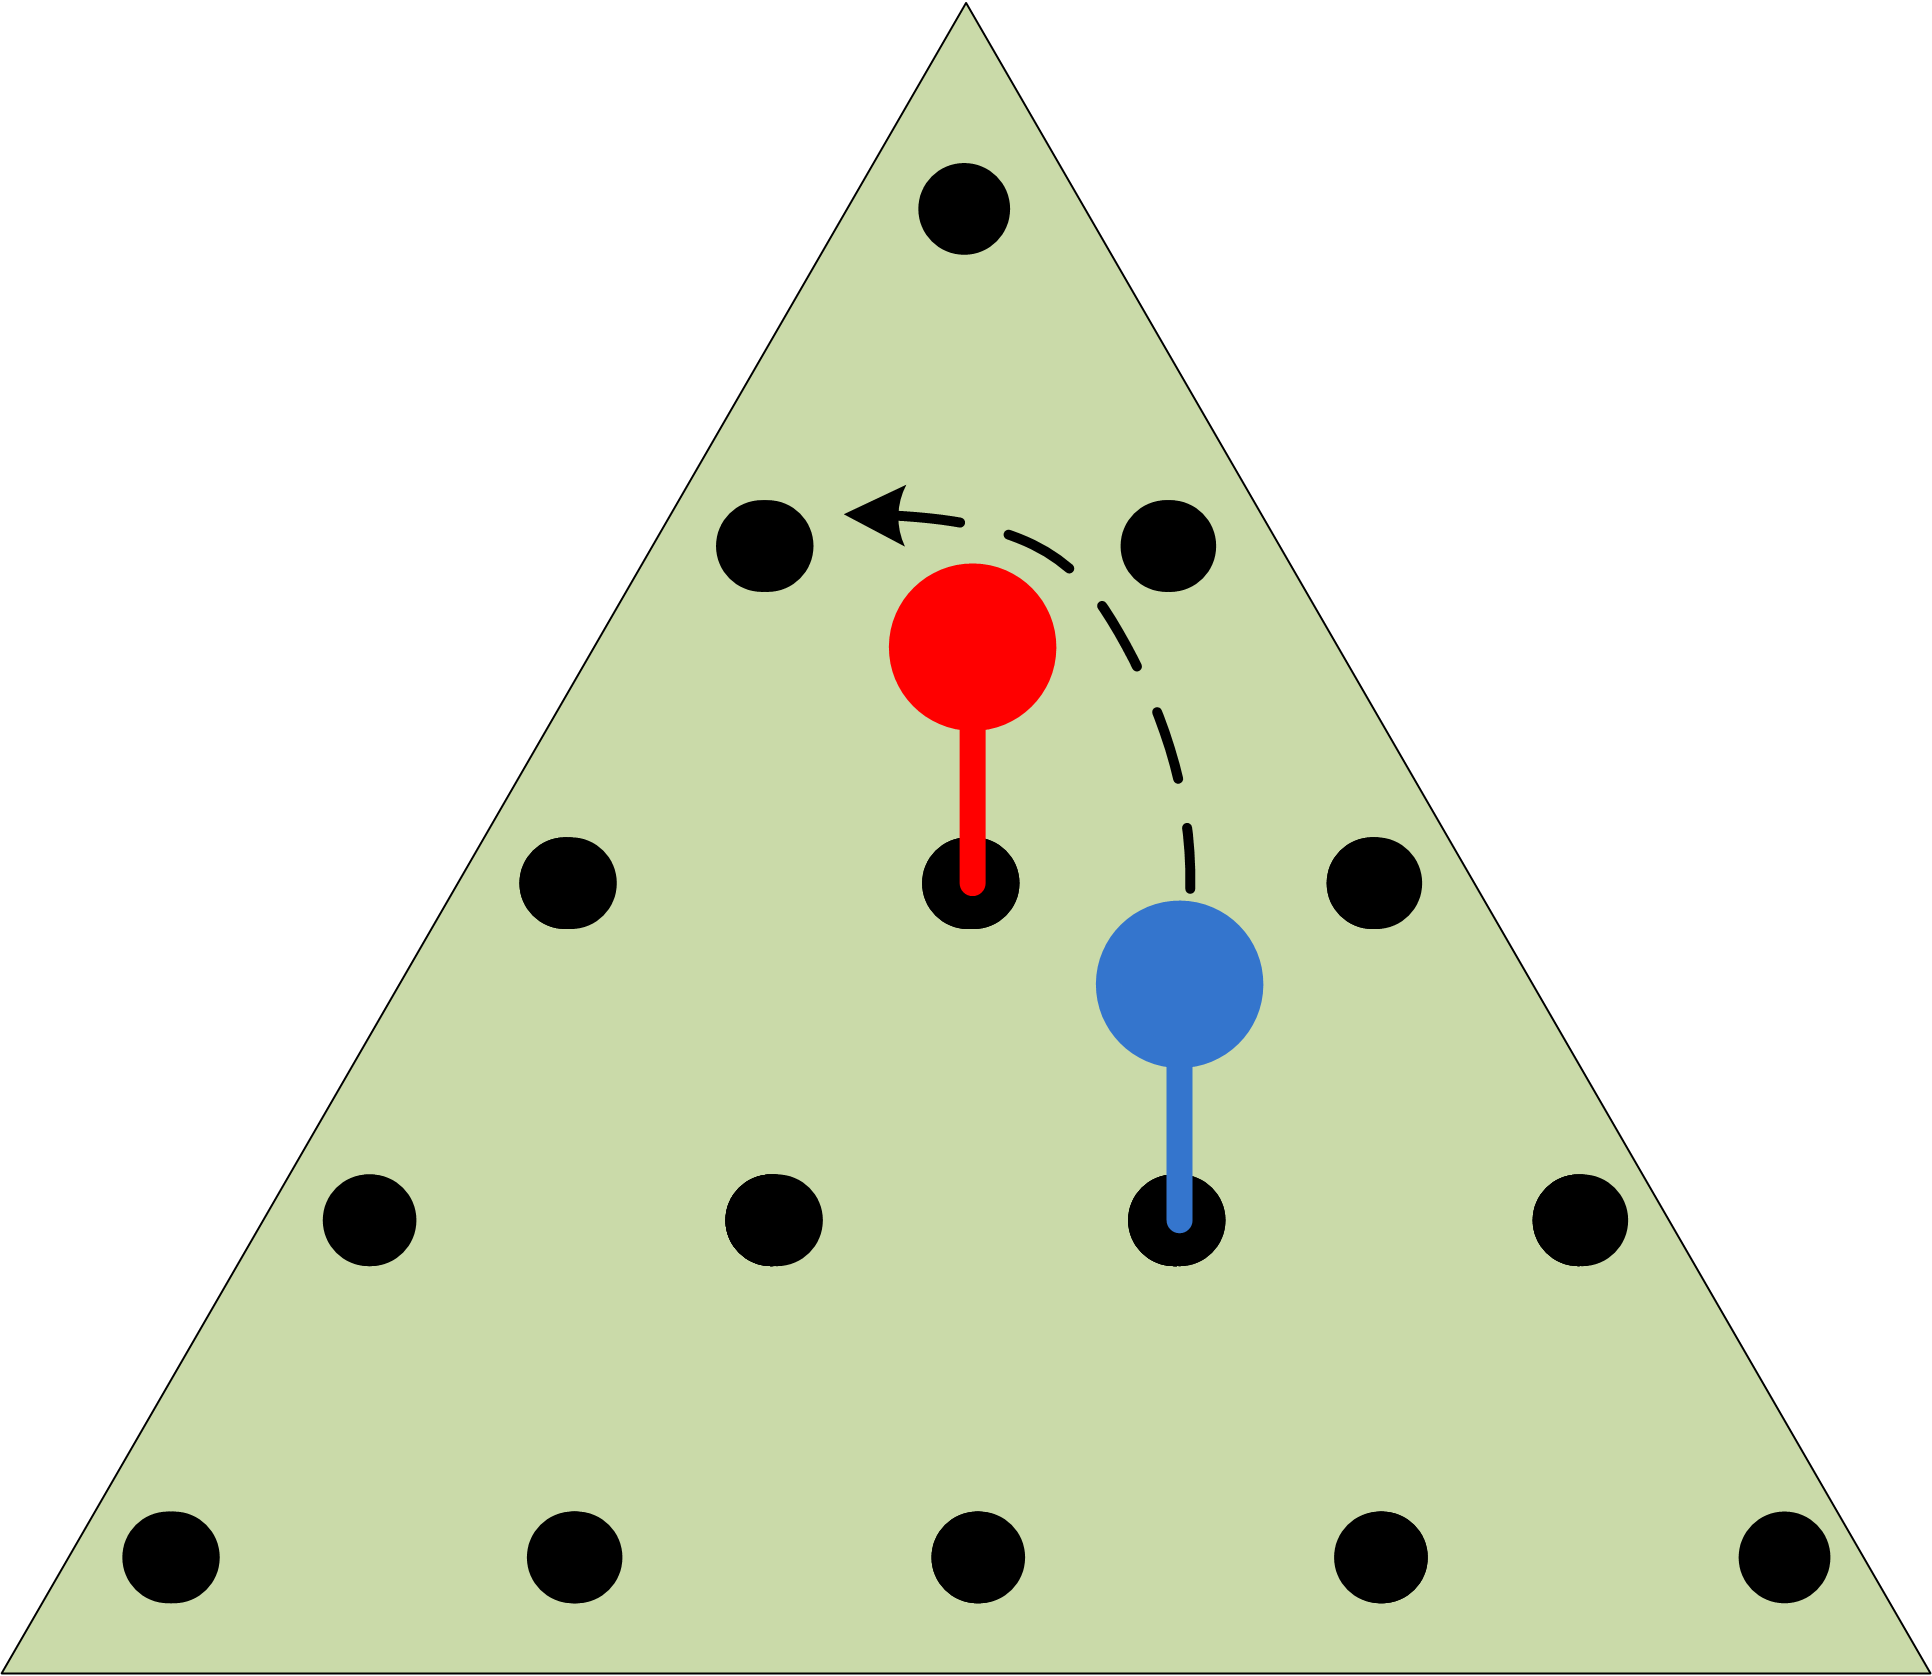
\includegraphics{figures/pegboard.png}}}}
\end{minipage}
\begin{minipage}[b]{0.35\linewidth}\vspace{0pt}\centering{
{\scalebox{0.40}{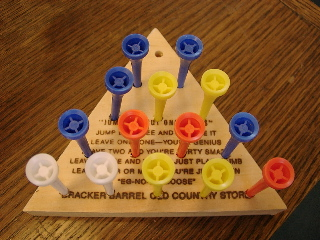
\includegraphics{images/pegboard.jpg}%I think I took this?
}}}
\end{minipage}
\caption{Pegboard Puzzle.\label{fig:pegboard}}
\subcap{The blue peg can jump the red peg as shown, removing the red peg.  The resulting position is a winning position.}
\end{center}
\end{figure}
 
Our goal is to develop a program that finds a winning solution to the pegboard game from any winnable starting position.  We use a \definition{brute force} approach: try all possible moves until we find one that works.  Brute force solutions only work on small-size problems.  Because they have to try all possibilities they are often too slow for solving large problems, even on the most powerful computers imaginable.\footnote{\cut{As we will see in \chintrac, }The generalized pegboard puzzle is an example of a class of problems known as \emph{NP-Complete}.  This means it is not known whether or not any solution exists that is substantially better than the brute force solution, but it would be extraordinarily surprising (and of momentous significance!) to find one.} 

The first thing to think about to solve a complex problem is what datatypes we need.  We want datatypes that represent the things we need to model in our problem solution.  For the pegboard game, we need to model the board with its pegs.  We also need to model actions in the game like a move (jumping over a peg).  The important thing about a datatype is what you can do with it.  To design our board datatype we need to think about what we want to do with a board.  In the physical pegboard game, the board holds the pegs.  The important property we need to observe about the board is which holes on the board contain pegs.  For this, we need a way of identifying board positions.  We define a datatype for representing positions first, then a datatype for representing moves, and a datatype for representing the board.  Finally, we use these datatypes to define a procedure that finds a winning solution.

\shortsection{Position} We identify the board positions using row and column numbers:
\begin{center}
     \scheme|(1 1)|\\
    \scheme|(2 1) (2 2)|\\
   \scheme|(3 1) (3 2) (3 3)|\\ 
  \scheme|(4 1) (4 2) (4 3) (4 4)|\\
 \scheme|(5 1) (5 2) (5 3) (5 4) (5 5)|\\
\end{center}

A position has a row and a column, so we could just use a Pair to represent a position.  This would work, but we prefer to have a more abstract datatype so we can think about a position's row and column, rather than thinking that a position is a Pair and using the \scheme|car| and \scheme|cdr| procedures to extract the row and column from the position.  

Our Position datatype should provide at least these operations:
\begin{procedurelist}
\item[\scheme|make-position|: Number $\times$ Number $\rightarrow$ Position] \forcenl Creates a Position representing the row and column given by the input numbers.
\item[\scheme|position-get-row|: Position $\rightarrow$ Number] \forcenl Outputs the row number of the input Position.
\item[\scheme|position-get-column|: Position $\rightarrow$ Number] \forcenl Outputs the column number of the input Position.
\end{procedurelist}

Since the Position needs to keep track of two numbers, a natural way to implement the Position datatype is to use a Pair.  A more defensive implementation of the Position datatype uses a \definition{tagged list}.  With a tagged list, the first element of the list is a tag denoting the datatype it represents.  All operations check the tag is correct before proceeding.  We can use any type to encode the list tag, but it is most convenient to use the built-in Symbol type. \index{general}{Symbol} Symbols are a quote (\scheme|'|) followed by a sequence of characters.  The important operation we can do with a Symbol, is test whether it is an exact match for another symbol using the \scheme|eq?| procedure.\index{general}{eq?}\label{ref:symbol} 

We define the tagged list datatype, \scheme|tlist|, using the \scheme|list-get-element| procedure from Example~\ref{example:list-get-element}:

\begin{schemedisplay}
(define (make-tlist tag p) (cons tag p))
(define (tlist-get-tag p) (car p))

(define (tlist-get-element tag p n)
  (if (eq? (tlist-get-tag p) tag)
      (list-get-element (cdr p) n)      
      (error (format "Bad tag: ~a (expected ~a)" 
                     (tlist-get-tag p) tag))))
\end{schemedisplay}

The \scheme|format| procedure is a built-in procedure similar to the \scheme|printf| procedure described in Section~\ref{sec:printing}.  Instead of printing as a side effect, \scheme|format| produces a String.  For example, \scheme|(format "list: ~a number: ~a." (list 1 2 3) 123)| evaluates to the String \schemeresult|"list: (1 2 3) number: 123."|. \index{general}{format}

This is an example of defensive programming.\index{general}{defensive programming}  Using our tagged lists, if we accidentally attempt to use a value that is not a Position as a position, we will get a clear  error message instead of a hard-to-debug error (or worse, an unnoticed incorrect result).

Using the tagged list, we define the Position datatype as:
\begin{schemedisplay}		
(define (make-position row col) (make-tlist 'Position (list row col)))
(define (position-get-row posn) (tlist-get-element 'Position posn 1))
(define (position-get-column posn) (tlist-get-element 'Position posn 2))
\end{schemedisplay}

Here are some example interactions with our Position datatype:
\begin{code}
\scheme|> (define pos (make-position 2 1))|\\
\scheme|> pos|\\
\schemeresult|(Position 2 1)|\\
\scheme|> (get-position-row pos)|\\
\schemeresult|2|\\
\scheme|> (get-position-row (list 1 2))|\\
\bugresult{Bad tag: 1 (expected Position)}\begin{aside}Error since input is not a Position.\end{aside}
\end{code}

\shortsection{Move}  A move involves three positions: where the jumping peg starts, the position of the peg that is jumped and removed, and the landing position.  One possibility would be to represent a move as a list of the three positions.  A better option is to observe that once any two of the positions are known, the third position is determined.  For example, if we know the starting position and the landing position, we know the jumped peg is at the position between them.  Hence, we could represent a jump using just the starting and landing positions.  

Another possibility is to represent a jump by storing the starting Position and the direction.  This is also enough to determine the jumped and landing positions.  This approach avoids the difficulty of calculating jumped positions.  To do it, we first design a Direction datatype for representing the possible move directions. Directions have two components: the change in the column (we use \scheme|1| for right and \scheme|-1| for left), and the change in the row (\scheme|1| for down and \scheme|-1| for up).  

We implement the Direction datatype using a tagged list similarly to how we defined Position:

\begin{schemedisplay}
(define (make-direction right down)    
   (make-tlist 'Direction (list right down)))
(define (direction-get-horizontal dir) (tlist-get-element 'Direction dir 1))
(define (direction-get-vertical dir) (tlist-get-element 'Direction dir 2))
\end{schemedisplay}

The Move datatype is defined using the starting position and the jump direction:
\begin{schemedisplay}
(define (make-move start direction) 
   (make-tlist 'Move (list start direction)))
(define (move-get-start move) (tlist-get-element 'Move move 1))
(define (move-get-direction move) (tlist-get-element 'Move move 2))
\end{schemedisplay}
We also define procedures for getting the jumped and landing positions of a move.  The jumped position is the result of moving one step in the move direction from the starting position.  So, it will be useful to define a procedure that takes a Position and a Direction as input, and outputs a Position that is one step in the input Direction from the input Position.
\begin{schemedisplay}
(define (direction-step pos dir)
  (make-position 
    (+ (position-get-row pos) (direction-get-vertical dir))
    (+ (position-get-column pos) (direction-get-horizontal dir))))
\end{schemedisplay}
Using \scheme|direction-step| we can implement procedure to get the middle and landing positions.
\begin{schemedisplay}
(define (move-get-jumped move) 
  (direction-step (move-get-start move) (move-get-direction move)))
(define (move-get-landing move) 
  (direction-step (move-get-jumped move) (move-get-direction move)))
\end{schemedisplay}

\shortsection{Board} The board datatype represents the current state of the board.  It keeps track of which holes in the board contain pegs, and provides operations that model adding and removing pegs from the board:
\begin{procedurelist}
\item[\scheme|make-board|: Number $\rightarrow$ Board] \forcenl Outputs a board full of pegs with the input number of rows.  (The standard physical board has 5 rows, but our datatype supports any number of rows.)
\item[\scheme|board-rows|: Board $\rightarrow$ Number] \forcenl Outputs the number of rows in the input board.
\item[\scheme|board-valid-position?|: Board $\times$ Position] $\rightarrow$ Boolean \forcenl Outputs \scheme|true| if input Position corresponds to a position on the Board; otherwise, \scheme|false|.
\item[\scheme|board-is-winning?|: Board $\rightarrow$ Boolean] \forcenl Outputs \scheme|true| if the Board represents a winning position (exactly one peg); otherwise, \scheme|false|.
\item[\scheme|board-contains-peg?|: Position $\rightarrow$ Boolean] \forcenl Outputs \scheme|true| if the hole at the input Position contains a peg; otherwise, \scheme|false|.
\item[\scheme|board-add-peg|: Board $\times$ Position $\rightarrow$ Board] \forcenl Output a Board containing all the pegs of the input Board and one additional peg at the input Position.  If the input Board already has a peg at the input Position, produces an error.
\item[\scheme|board-remove-peg|: Board $\times$ Position $\rightarrow$ Board] \forcenl Outputs a Board containing all the pegs of the input Board except for the peg at the input Position.  If the input Board does not have a peg at the input Position, produces an error.
\end{procedurelist}

The procedures for adding and removing pegs change the state of the board to reflect moves in the game, but nothing we have seen so far, however, provides a means for changing the state of an existing object.\footnote{We will introduce mechanisms for changing state in Chapter~\ref{ch:state}.  Allowing state to change breaks the substitution model of evaluation.}  So, instead of defining these operations to change the state of the board, they actually create a new board that is different from the input board by the one new peg.  These procedures take a Board and Position as inputs, and produce as output a Board.

There are lots of different ways we could represent the Board.  One possibility is to keep a List of the Positions of the pegs on the board.  Another possibility is to keep a List of the Positions of the empty holes on the board.  Yet another possibility is to keep a List of Lists, where each List corresponds to one row on the board.  The elements in each of the Lists are Booleans representing whether or not there is a peg at that position.  The good thing about data abstraction is we could pick any of these representations and change it to a different representation later (for example, if we needed a more efficient board implementation).  As long as the procedures for implementing the Board are updated the work with the new representation, all the code that uses the board abstraction should continue to work correctly without any changes.

We choose the third option and represent a Board using a List of Lists where each element of the inner lists is a Boolean indicating whether or not the corresponding position contains a peg.  So, \scheme|make-board| evaluates to a List of Lists, where each element of the List contains the row number of elements and all the inner elements are \schemeresult|true| (the initial board is completely full of pegs).  First, we define a procedure \scheme|make-list-of-constants| that takes two inputs, a Number, \scheme|n|, and a Value, \scheme|val|.  The output is a List of length \scheme|n| where each element has the value \scheme|val|.
\begin{schemedisplay}
(define (make-list-of-constants n val)
  (if (= n 0) null (cons val (make-list-of-constants (- n 1) val))))
\end{schemedisplay}
To make the initial board, we use \scheme|make-list-of-constants| to make each row of the board.  As usual, a recursive problem solving strategy works well: the simplest board is a board with zero rows (represented as the empty list); for each larger board, we add a row with the right number of elements.  

The tricky part is putting the rows in order.  This is similar to the problem we faced with \scheme|intsto|, and a similar solution using \scheme|append-list| works here:
\begin{schemedisplay}
(define (make-board rows) 
  (if (= rows 0) null
      (list-append (make-board (- rows 1)) 
                   (list (make-list-of-constants rows true)))))
\end{schemedisplay}

Evaluating \scheme|(make-board 3)| produces \scheme|((true) (true true) (true true true))|.

The \scheme|board-rows| procedure takes a Board as input and outputs the number of rows on the board.
\begin{schemedisplay}
(define (board-rows board) (length board))
\end{schemedisplay}

The \scheme|board-valid-position?| indicates if a Position is on the board.  A position is valid if its row number is between 1 and the number of rows on the board, and its column numbers is between 1 and the row number.
\begin{schemedisplay}
(define (board-valid-position? board pos)
  (and (>= (position-get-row pos) 1) (>= (position-get-column pos) 1)
       (<= (position-get-row pos) (board-rows board))
       (<= (position-get-column pos) (position-get-row pos))))
\end{schemedisplay}

We need a way to check if a Board represents a winning solution (that is, contains only one peg).  We implement a more general procedure to count the number of pegs on a board first.  Our board representation used \scheme|true| to represent a peg.  To count the pegs, we first map the Boolean values used to represent pegs to \scheme|1| if there is a peg and \scheme|0| if there is no peg.  Then, we use \scheme|sum-list| to count the number of pegs.  Since the Board is a List of Lists, we first use \scheme|list-flatten| to put all the pegs in a single List.
\begin{schemedisplay}
(define (board-number-of-pegs board)
  (list-sum
   (list-map (lambda (peg) (if peg 1 0)) (list-flatten board))))
\end{schemedisplay}
A board is a winning board if it contains exactly one peg:
\begin{schemedisplay}
(define (board-is-winning? board) 
   (= (board-number-of-pegs board) 1))
\end{schemedisplay}

The \scheme|board-contains-peg?| procedure takes a Board and a Position as input, and outputs a Boolean indicating whether or not that Position contains a peg.   To implement \scheme|board-contains-peg?| we need to find the appropriate row in our board representation, and then find the element in its list corresponding to the position's column.  The \scheme|list-get-element| procedure (from Example~\ref{example:list-get-element}) does exactly what we need.  Since our board is represented as a List of Lists, we need to use it twice: first to get the row, and then to select the column within that row:
\begin{schemedisplay}
(define (board-contains-peg? board pos)
  (list-get-element (list-get-element board (position-get-row pos)) 
                    (position-get-column pos)))
\end{schemedisplay}
Defining procedures for adding and removing pegs from the board is more complicated.  Both of these procedures need to make a board with every row identical to the input board, except the row where the peg is added or removed.  For that row, we need to replace the corresponding value.  Hence, instead of defining separate procedures for adding and removing we first implement a more general \scheme|board-replace-peg| procedure that takes an extra parameter indicating whether a peg should be added or removed at the selected position.

First we consider the subproblem of replacing a peg in a row.  The procedure \scheme|row-replace-peg| takes as input a List representing a row on the board and a Number indicating the column where the peg should be replaced.  We can define \scheme|row-replace-peg| recursively: the base case is when the modified peg is at the beginning of the row (the column number is \scheme|1|); in the recursive case, we copy the first element in the List, and replace the peg in the rest of the list.  The third parameter indicates if we are adding or removing a peg.  Since \scheme|true| values represent holes with pegs, a \scheme|true| value indicates that we are adding a peg and \scheme|false| means we are removing a peg.
\begin{schemedisplay}
(define (row-replace-peg pegs col val)
  (if (= col 1) 
      (cons val (cdr pegs))
      (cons (car pegs) (row-replace-peg (cdr pegs) (- col 1) val))))
\end{schemedisplay}

To replace the peg on the board, we use \scheme|row-replace-peg| to replace the peg on the appropriate row, and keep all the other rows the same.  
\begin{schemedisplay}
(define (board-replace-peg board row col val)
  (if (= row 1) 
      (cons (row-replace-peg (car board) col val) (cdr board))
      (cons (car board) (board-replace-peg (cdr board) (- row 1) col val))))
\end{schemedisplay}

Both \scheme|board-add-peg| and \scheme|board-remove-peg| can be defined simply using \scheme|board-remove-peg|.  They first check if the operation is valid (adding is valid only if the selected position does not contain a peg, removing is valid only if the selected position contains a peg), and then use \scheme|board-replace-peg| to produce the modified board:
\begin{schemedisplay}
(define (board-add-peg board pos)
  (if (board-contains-peg? board pos)
      (error (format "Board already contains peg at position: ~a" pos))
      (board-replace-peg board (position-get-row pos) 
                               (position-get-column pos) true)))

(define (board-remove-peg board pos)
  (if (not (board-contains-peg? board pos))
      (error (format "Board does not contain peg at position: ~a" pos))
      (board-replace-peg board (position-get-row pos) 
                               (position-get-column pos) false)))
\end{schemedisplay}

We can now define a procedure that models making a move on a board.  Making a move involves removing the jumped peg and moving the peg from the starting position to the landing position.  Moving the peg is equivalent to removing the peg from the starting position and adding a peg to the landing position, so the procedures we defined for adding and removing pegs can be composed to model making a move.  We add a peg landing position to the board that results from removing the pegs in the starting and jumped positions:
\begin{schemedisplay}
(define (board-execute-move board move)
  (board-add-peg 
   (board-remove-peg 
    (board-remove-peg board (move-get-start move)) 
    (move-get-jumped move))
   (move-get-landing move)))
\end{schemedisplay}

\shortsection{Finding Valid Moves}
Now that we can model the board and simulate making jumps, we are ready to develop the solution.  At each step, we try all valid moves on the board to see if any move leads to a winning position (that is, a position with only one peg remaining).  So, we need a procedure that takes a Board as its input and outputs a List of all valid moves on the board.  We break this down into the problem of producing a list of all conceivable moves (all moves in all directions from all starting positions on the board), filtering that list for moves that stay on the board, and then filtering the resulting list for moves that are legal (start at a position containing a peg, jump over a position containing a peg, and land in a position that is an empty hole). 

First, we generate all conceivable moves by creating moves starting from each position on the board and moving in all possible move directions.  We break this down further: the first problem is to produce a List of all positions on the board.  

We can generate a list of all row numbers using the \scheme|intsto| procedure (from Example~\ref{example:intsto}).  To get a list of all the positions, we need to produce a list of the positions for each row.  We do this by mapping each row to the corresponding list:
\begin{schemedisplay}
(define (all-positions-helper board)
  (list-map 
    (lambda (row) (list-map (lambda (col) (make-position row col))
                            (intsto row)))
    (intsto (board-rows board)))
\end{schemedisplay}
This almost does what we need, except instead of producing one List containing all the positions, it produces a List of Lists for the positions in each row.  The \scheme|list-flatten| procedure (from Example~\ref{example-list-flatten}) produces a flat list containing all the positions.
\begin{schemedisplay}          
(define (all-positions board)
  (list-flatten (all-positions-helper board)))
\end{schemedisplay}

For each Position, we find all possible moves starting from that position.  We can move in six possible directions on the board: left, right, up-left, up-right, down-left, and down-right.
\begin{schemedisplay}
(define all-directions
  (list 
   (make-direction -1 0) (make-direction 1 0) ; left, right
   (make-direction -1 -1) (make-direction 0 -1) ; up-left, up-right
   (make-direction 0 1) (make-direction 1 1))) ; down-left, down-right
\end{schemedisplay}

For each position on the board, we create a list of possible moves starting at that position and moving in each possible move directions.  This produces a List of Lists, so we use \scheme|list-flatten| to flatten the output of the \scheme|list-map| application into a single List of Moves.

\begin{schemedisplay}
(define (all-conceivable-moves board)
  (list-flatten
    (list-map
      (lambda (pos) (list-map (lambda (dir) (make-move pos dir))
                              all-directions))
      (all-positions board))))
\end{schemedisplay}

The output produced by \scheme|all-conceivable-moves| includes moves that fly off the board.  We use the \scheme|list-filter| procedure to remove those moves, to get the list of moves that stay on the board:
\begin{schemedisplay}
(define (all-board-moves board)
  (list-filter 
   (lambda (move) (board-valid-position? board (move-get-landing move)))          
   (all-conceivable-moves board)))
\end{schemedisplay}
Finally, we need to filter out the moves that are not legal moves.  A legal move must start at a position that contains a peg, jump over a position that contains a peg, and land in an empty hole.  We use \scheme|list-filter| similarly to how we kept only the moves that stay on the board:
\begin{schemedisplay}
(define (all-legal-moves board)
  (list-filter
    (lambda (move)
      (and 
       (board-contains-peg? board (move-get-start move))
       (board-contains-peg? board (move-get-jumped move))
       (not (board-contains-peg? board (move-get-landing move)))))
   (all-board-moves board)))
\end{schemedisplay}

\shortsection{Winning the Game}
Our goal is to find a sequence of moves that leads to a winning position, starting from the current board.  If there is a winning sequence of moves, we can find it by trying all possible moves on the current board.  Each of these moves leads to a new board.  If the original board has a winning sequence of moves, at least one of the new boards has a winning sequence of moves.  Hence, we can solve the puzzle by recursively trying all moves until finding a winning position.
\begin{schemedisplay}
(define (solve-pegboard board)
  (if (board-is-winning? board)
      null ; no moves needed to reach winning position
      (try-moves board (all-legal-moves board))))
\end{schemedisplay}
If there is a sequence of moves that wins the game starting from the input Board, \scheme|solve-pegboard| outputs a List of Moves representing a winning sequence.  This could be \schemeresult|null|, in the case where the input board is already a winning board.  If there is no sequence of moves to win from the input board, \scheme|solve-pegboard| outputs \schemeresult|false|.

It remains to define the \scheme|try-moves| procedure.  It takes a Board and a List of Moves as inputs.  If there is a sequence of moves that starts with one of the input moves and leads to a winning position it outputs a List of Moves that wins; otherwise, it outputs \schemeresult|false|.

The base case is when there are no moves to try.  When the input list is \scheme|null| it means there are no moves to try.  We output \scheme|false| to mean this attempt did not lead to a winning board.  Otherwise, we try the first move.  If it leads to a winning position, \scheme|try-moves| should output the List of Moves that starts with the first move and is followed by the rest of the moves needed to solve the board resulting from taking the first move (that is, the result of \scheme|solve-pegboard| applied to the Board resulting from taking the first move).  If the first move doesn't lead to a winning board, it tries the rest of the moves by calling \scheme|try-moves| recursively.
\begin{schemedisplay}
(define (try-moves board moves)
  (if (null? moves)
      false ; didn't find a winner 
      (if (solve-pegboard (board-execute-move board (car moves)))
          (cons (car moves) 
                (solve-pegboard (board-execute-move board (car moves))))
          (try-moves board (cdr moves)))))
\end{schemedisplay}

Evaluating \scheme|(solve-pegboard (make-board 5))| produces \schemeresult|false| since there is no way to win starting from a completely full board.  Evaluating \scheme|(solve-pegboard (board-remove-peg (make-board 5) (make-position 1 1)))| takes about three minutes to produce this sequence of moves for winning the game starting from a 5-row board with the top peg removed:
\begin{schemedisplay}
((Move (Position 3 1) (Direction 0 -1))
 (Move (Position 3 3) (Direction -1 0))
 (Move (Position 1 1) (Direction 1 1))
 (Move (Position 4 1) (Direction 0 -1))
 ... ; 8 moves elided
 (Move (Position 5 1) (Direction 1 1)))
\end{schemedisplay}

 %(Move (Position 4 4) (Direction -1 -1))
 %(Move (Position 5 2) (Direction 0 -1))
 %(Move (Position 5 3) (Direction 0 -1))
 %(Move (Position 2 1) (Direction 1 1))
 %(Move (Position 2 2) (Direction 1 1))
 %(Move (Position 5 5) (Direction -1 -1))
 %(Move (Position 3 3) (Direction 0 1))
 %(Move (Position 5 4) (Direction -1 0))
\begin{subexerciselist}
\item \goldstar Change the implementation to use a different Board representation, such as keeping a list of the Positions of each hole on the board.  Only the procedures with names starting with \scheme|board-| should need to change when the Board representation is changed.  Compare your implementation to this one.

\item \goldstar The standard pegboard puzzle uses a triangular board, but there is no reason the board has to be a triangle.  Define a more general pegboard puzzle solver that works for a board of any 
 shape.

\item \doublegoldstar The described implementation is very inefficient.  It does lots of redundant computation.  For example, \scheme|all-possible-moves| evaluates to the same value every time it is applied to a board with the same number of rows.  It is wasteful to recompute this over and over again to solve a given board.  See how much faster you can make the pegboard solver.  Can you make it fast enough to solve the 5-row board in less than half the original time?  Can you make it fast enough to solve a 7-row board?
\end{subexerciselist}

} % end exploration

\section{Summary of Part I}

To conclude Part I, we revisit the three main themes introduced in Section~\ref{sec:roadmap}.

\emph{Recursive definitions.}\index{general}{recursive definition}  We have seen many types of recursive definitions and used them to solve problems, including the pegboard puzzle.  Recursive grammars provide a compact way to define a language; recursive procedure definitions enable us to solve problems by optimistically assuming a smaller problem instance can be solved and using that solution to solve the problem; recursive data structures such as the list type allow us to define and manipulate complex data built from simple components.  All recursive definitions involve a base case.  For grammars, the base case provides a way to stop the recursive replacements by produce a terminal (or empty output) directly; for procedures, the base case provides a direct solution to a small problem instance; for data structures, the base case provides a small instance of the data type (e.g., \scheme|null|).  We will see many more examples of recursive definitions in the rest of this book.

\emph{Universality.}\index{general}{universality} All of the programs we have can be created from the simple subset of Scheme introduced in Chapter~\ref{ch:programming}.  This subset is a \definition{universal programming language}: it is powerful enough to describe all possible computations.  We can generate all the programs using the simple Scheme grammar, and interpret their meaning by systematically following the evaluation rules.  We have also seen the universality of code and data.  Procedures can take procedures as inputs, and produce procedures as outputs.  

\emph{Abstraction.}\index{general}{abstraction} Abstraction hides details by giving things names.  Procedural abstraction defines a procedure; by using inputs, a short procedure definition can abstract infinitely many different information processes.  Data abstraction hides the details of how data is represented by providing procedures that abstractly create and manipulate that data.  As we develop programs to solve more complex problems, it is increasingly important to use abstraction well to manage complexity.  We need to break problems down into smaller parts that can be solved separately.  Solutions to complex problems can be developed by thinking about what objects need to be modeled, and designing data abstractions the implement those models.  Most of the work in solving the problem is defining the right datatypes; once we have the datatypes we need to model the problem well, we are usually well along the path to a solution.

With the tools from Part I, you can define a procedure to do any possible computation.  In Part II, we examine the costs of executing procedures.
\end{schemeregion}

